\section{Sensibility Testbed Design}\label{sec-design}

This section describes the design of the Sensibility Testbed. 
%On one hand, Sensibility Testbed manages how device owners make their
%devices accessible to the research community. On the other hand,
%it offers technical resources to researchers that allow them to
%securely collect data from remote mobile devices. 
We start with
an overview of the testbed infrastructure (Section~\ref{sec-overview}), 
and a description of each testbed component 
(Section~\ref{sec-component}), then finally a discussion of how all the 
components work together to assist experimenters' experimentation,
and protect device owners' personal information 
(Section~\ref{sec-scenario}).


\subsection{Overview}\label{sec-overview}

%\subsubsection{Interacting Parties}\label{sec-parties}
In Sensibility Testbed, there are three types of interacting
parties, as shown in Figure~\ref{fig-arch}: mobile \textit{devices} 
owned by ordinary people, with our app installed; a 
\textit{clearinghouse} server that discovers and configures
participating devices; and \textit{experimenters} who want to run
experiments on mobile devices. 

\begin{figure}
\center{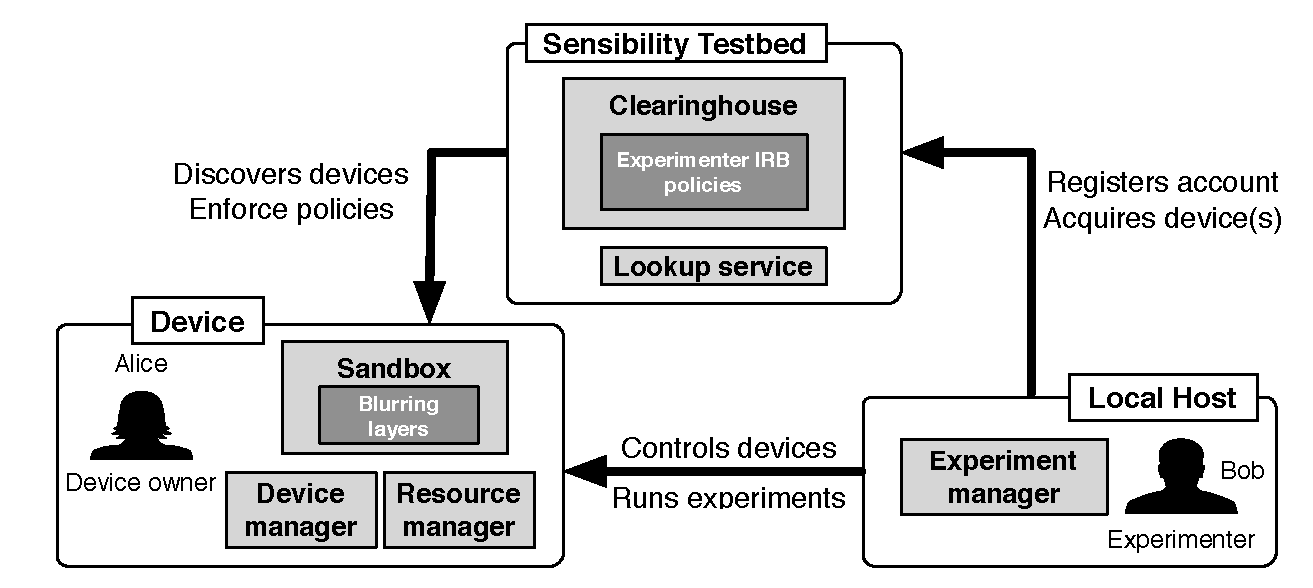
\includegraphics[width=\columnwidth]{figs/arch.pdf}}
%\vspace*{-20pt}
\caption{\small Sensibility Testbed architecture. \label{fig-arch}}
\end{figure}

Mobile devices
provide resources and data for researchers to use in their
experiments. In order to perform safe experiments on mobile
devices, a researcher must provide to the clearinghouse server
the IRB policies from his institute for accessing devices 
(Section~\ref{sec-ch}). \yanyan{need a screenshot} These 
policies restrict what and how data can be accessed by the 
researcher. The
clearinghouse server helps the researcher acquire and manage
devices, and also codifies the policies specified by the
researcher's IRB into data blurring layers that are enforced on
mobile devices. Such a process can protect device
owners' personal information. After obtaining remote sandboxes
and having IRB policies in place, researchers can perform
experiments on the devices directly, using their credentials assigned by
the clearinghouse. Researchers' code runs in a sandbox 
that isolates the code from the rest of the device
host system (Section~\ref{sec-repy}). To control the execution of 
code, the researcher uses a local machine to manage the 
experiments via an experiment manager. This tool can deploy 
and run experiments in sandboxes on remote devices that are 
acquired through the clearinghouse (Section~\ref{sec-emt}).

%\subsubsection{Enforcing IRB Approved Policies}


\subsection{Testbed Components}\label{sec-component}

The components of the Sensibility Testbed are shown in Figure~\ref{fig-arch}.
They are central to the operation of the testbed. 
In this section, we describe the function of each component: the
software running on a mobile device, the clearinghouse~\cite{ch}, 
and experiment manager.

\subsubsection{Device Software}\label{sec-repy}

%In Sensibility Testbed, all experiments execute in a secure 
%sandbox on the end devices.
%Experimenters' code executes in a sandbox that isolates the 
%experiment code from the device host system. 
Sensibility Testbed uses a sandbox called Repy (Restricted 
Python)\footnote{\scriptsize This is the 
same security-reviewed sandbox~\cite{cappos2010retaining} used in
our prior work, the Seattle testbed~\cite{seattle}. This sandbox
mitigates the impact of bugs in experimenter code.}, which 
provides security isolation and performance isolation on mobile devices.
%Instead of developing full-fledged Android apps, all 
%experiments in Sensibility Testbed are written in a language
%similar to Python, and run in a secure %Python-based
Experimenters use a Python-like programming interface~\cite{repyv2}
to write experiment code, upload the code and execute it in the
sandbox. The programming interface includes functions for networking, 
file system, threading, locking, logging, and so on. To access sensors, 
the sandbox also has a set of sensor functions~\cite{sensors}. The
details about the implementation of the Repy sandbox are described 
in Section~\ref{sec-repy-ext}.

To install Repy and other software on a device, a device owner downloads 
our Sensibility Testbed app from the Google Play Store \cite{sensibility-app}.
The app displays a consent form, \yanyan{cite link} where the device owner can review
the testbed's general usage policy \yanyan{cite link} and must 
agree to before the installation. If the device owner gives his
consent, the device will be installed with the Repy sandbox, the native Android code to 
start or stop the sandbox, and an interface to communicate with the testbed 
infrastructure, particularly the clearinghouse (described below). 
By agreeing to our general usage policy, device 
owners of different ages, from different countries, with different
background need only to opt in \textit{once} to our testbed as 
volunteers (during the time of app installation). As a result, an 
experimenter who wants to conduct a research experiment 
%requests devices through our clearinghouse, which assigns 
%them devices from a set of available resources. As a result, 
%the researcher
does not need to get consent from each subject for each individual
experiment. The testbed thus reduces the burden from both the 
device owners and experimenters. 

%However, the current Repy sandbox does not include calls to access sensors. 
%%To obtain the sensor data, we need to extend the sandbox. 
%The extended Repy sandbox that allows sensor access  
%will be described in Section~\ref{sec-repy-ext}.
Furthermore, the Repy sandbox allows us to change the 
behavior of its programming interface, and control the 
data gathered from the device. 
%For  an experiment
%that involves GPS location, a privacy policy might restrict the
%level of data granularity available to the experiment. For example, it can
%obfuscate GPS location such that it only identifies the center
%of the city that the device is located in, rather than the exact
%location. Using the same technique, 
To illustrate, the IP address of a device may be anonymized, 
the frequency to access GPS location can be constrained, and 
access to camera can be disabled, and so on. 
%Such privacy protection is a contribution of Sensibility Testbed, 
%which does not exist in any prior work. 
The details of policy implementation are presented in 
Section~\ref{sec-layer} and \ref{sec-nanny}.

\subsubsection{Clearinghouse}\label{sec-ch}
The clearinghouse~\cite{ch} is a testbed server that keeps 
track of devices and mediates experimenter access to the 
available devices. It allows experimenters to register 
accounts and share access to a common pool of devices.
It does so by looking up available devices, and assigning
them to researcher's experiment account upon request. 
Its key role is to facilitate device sharing, 
which relieves individual experimenters from repeatedly 
recruiting devices for each experiment.

%The clearinghouse
%plays an intermediate role between the experimenter and 
%the device owner.
%As described in Section~\ref{sec-overview}, when an 
%experimenter registers at the clearinghouse, he
%needs to provide his IRB policies. These policies ensure that
%the researcher cannot conduct experiments to access data that
%extend beyond the experiment policy. The clearinghouse 
%translates and codifies each policy, and instructs the 
%sandboxes on remote devices to implement these policies. 
%When experiment code is running in the sandbox, the 
%policies will be applied to restrict %the precision of sensor 
%%data or the frequency to access 
%sensor access. 
In order to obtain an IRB approval, a researcher first fills out an experiment
registration form \yanyan{cite url or show screenshot} at the 
clearinghouse. The clearinghouse website shows 
a list of available sensors, and each of their required accuracy 
and access frequency. Aftering filling out this form, the researcher uses it as 
a template to submit and apply for IRB approval at his or her institution. 
This form serves as a reference document, along with details about 
Sensibility Testbed,\yanyan{cite our docs} to reduce the researcher's burden. 

After the application is submitted, the researcher's IRB may disagree with 
the initial experiment requirement. %For example, Bob wants to access cell 
%IDs in cellular networks, but his IRB disallows such data access. Bob then
The researcher then revises the experiment requirement, obtains IRB approval, and
submits the revised experiment registration form to the clearinghouse. Finally, the clearinghouse
parses the registration form, extracts each data accuracy and access 
frequency approved by the researcher's IRB, and assigns an experiment 
account to the researcher. Once the researcher requests 
devices, the clearinghouse supplies the extracted data as input parameters to
the blurring layers that will be instantiated on the requested devices. The clearinghouse
has a default set of blurring layers for each sensor, each have the 
sensor's accuracy and access frequency as parameters. The details about
how each policy is implemented will be introduced in Section~\ref{sec-policy}.

This Sensibility Testbed
clearinghouse protocol for research plays a central role in
easing the device recruitment and experiment setup for experimenters, 
and ensures the enforcement
of privacy policy\footnote{\scriptsize The Sensibility Testbed Clearinghouse
protocol for research with human subjects has been approved by
the IRB at New York University (IRB \# 15-10751).}. 

\subsubsection{Experiment Manager}\label{sec-emt}

To run code remotely on mobile devices, an experimenter uses an
experiment manager from his local machine 
%which contains Bob's private key, \path{key.bob-priv}, 
to access the sandboxes on the remote devices assigned by the clearinghouse. 
This experiment manager is a light-weight command line 
console~\cite{demo-kit} that allows direct access from the 
experimenter's local machine to a set of remote devices. 
The clearinghouse is not involved when the experimenter deploys 
an experiment and runs the code, and it does not store any
data on the experimenter's behalf. After collecting the data he needs, the
experimenter can use the experiment manager to download data from the remote devices. 
Alternatively, the experimenter can set up his own server to store all 
the data\footnote{\scriptsize
If an experimenter stores data at his own server, he must use protective
measures to ensure that the data sent from the mobile devices is
properly encrypted, and the server storage cannot be tampered
with by any other parties. For example, the experimenter needs to register
his server by providing the server's certificate and URL to our
clearinghouse. The clearinghouse then instructs the devices
accessible to the experimenter that all the sensor data collected should be
sent to this server. The sandboxes on these devices then issue
\texttt{HTTPS POST} using the server's certificate, and send encrypted
data to the experimenter's server. After the data is collected, how to store
the data securely is mandated by the experimenter's IRB.}, or use a data 
store service we provide (a service called Sensevis~\cite{sensevis}, 
not shown in Figure~\ref{fig-arch}).

\smallskip
In summary, 
%Prior to running an experiment on Sensibility Testbed, a
%experimenter first fills out a form in plain text to describe the
%purpose of the research experiment. This experiment description
%is created at the Sensibility Testbed clearinghouse
%where the researcher indicates the type of data to be collected,
%how that data will be used and stored, and so on. 
%
%Once this information is collected from the researcher, the
%clearinghouse automatically generates a set of blurring layers
%that implements the experiment policy (Section~\ref{sec-policy}). In
%Sensibility Testbed, researchers can collect data from the
%sensors on the device, such as GPS, Bluetooth, battery
%information, accelerometer, light, and orientation,
%etc. The blurring layers we provide consist of
%data access restrictions, created in accordance with
%researcher's experiment description, by using the Sensibility
%Testbed's sandboxing technique 
%(Section~\ref{sec-repy})~\cite{cappos2010retaining}. These restrictions ensure that
%the researcher cannot conduct experiments to access data that
%extend beyond the experiment policy. 
%
%This Sensibility Testbed
%clearinghouse protocol for research plays a central role in
%easing the approval process of IRB, and ensures the enforcement
%of privacy policy\footnote{The Sensibility Testbed Clearinghouse
%protocol for research with human subjects has been approved by
%the IRB at New York University. \yanyan{might need a link to
%your approval letter or ref number}}. 
using Sensibility Testbed, device owners' privacy is protected
from any inadvertent or malicious attempt, and experimenters 
are able to go through a streamlined process of device 
recruitment and experiment setup.

%the device owners do not need to give consents 
%multiple times, to each project of each researcher. 
In the following, we present several use cases to
demonstrate how device owners opt in as volunteers, and how
researchers do experiments on devices without compromising device
owners' privacy.

\subsection{Testbed Scenarios}\label{sec-scenario}
%\yanyan{should this section go after policies?}
To demonstrate how Sensibility Testbed's components interact with
each other to assist experimenter's experimentation, this section will go
through several scenarios. In these scenarios, a smartphone owner, Alice,
participates in the testbed; an experimenter, Bob, runs code on
Sensibility Testbed using Alice's smartphone, among other
devices discovered. Specifically, Bob wants to know the cellular service
quality in major cities. As such, he needs location information
of individual devices, their cellular service provider, network
type (3G, 4G, LTE, etc.), and signal strength.

Note that in Sensibility Testbed, there are two types of keys. A device
owner has an \textit{identification key} to identify the app installed on a 
device. An experimenter has a pair of public/private \textit{authentication 
keys} to authenticate the experimenter with the clearinghouse and 
the set of devices that he has access to.

\textbf{Smartphone owner participates in the testbed.}
%\label{sec-owner-participate}
When Alice, a smartphone owner, decides to participate in
Sensibility Testbed, she first downloads and installs our Sensibility Testbed
app~\cite{sensibility-app}. %which currently supports Android devices.
%This app contains a testbed key \path{key.sensibility} used for 
%device discovery (similar to a device owner's identification key). 
%the Repy sandbox (Section~\ref{sec-repy}), 
%and native Android code to handle user interaction, communicate 
%with the clearinghouse, and so on. 
%Before installation, the app displays a
%consent form to Alice. If Alice
%agrees to the terms and policy, the app will be installed on her
%device. 
Once the app is started, Alice's device can be
discovered by the clearinghouse. Her device periodically contacts 
a lookup service to advertise itself to Sensibility Testbed. 
A lookup service is a distributed key-value store, such as a DHT, that 
allows one to retrieve values associated with keys and to associate 
keys with values. 

To keep track of Alice's device, the
clearinghouse periodically queries the lookup service to
discover any new devices. Once Alice's device is discovered, the
clearinghouse obtains its identification key \path{key.alice} generated
during installation, and stores this key. 
%clearinghouse uses a database that stores her device's unique
%identification key, \path{key.alice}, generated during installation. 
This key is not associated with Alice's or her
device's identity, but only the app's installation on the device. If
Alice uninstalls the Sensibility app, \path{key.alice} is
deleted at the clearinghouse, which effectively unlinks
her device from any metadata stored on the clearinghouse.
Instead of uninstalling, Alice may also choose to opt out of
individual experiments.

\textbf{Researcher provides IRB policies.}
%\label{sec-irb-policy}
To run code on Sensibility Testbed, experimenter Bob provides a
set of detailed IRB policies from his institution. The process of how
Bob obtains such policies is described in Section~\ref{sec-ch}.
Bob first fills out an experiment registration form and specifies that 
%what data can be accessed by a research experiment, at which 
%granularity or frequency such data can be accessed, how data 
%should be securely stored, and so on. \yanyan{cite register 
%experiment website url.}
his experiment can (1) read location information
from devices at the granularity of a city, (2) read accurate
cellular signal strength and network type, as well as
%but not allow access to information about 
cell IDs, and (3) get location and
cellular network data updates every 10 minutes. 
%Bob submits an
%experiment description for these requirements, which the
%clearinghouse will codify into policies that are later enforced
%on remote mobile devices (Section~\ref{sec-ch}).
Bob then uses this form, along with details about Sensibility Testbed, 
to apply for IRB approval at his institution.

After the application is submitted, Bob's IRB disagrees that his 
experiment should access cell IDs in cellular networks, but approves 
the rest. Bob then ubmits the revised experiment registration form
and his IRB approval, and obtains an experiment account at the
clearinghouse, and his authentication keys assigned by the 
clearinghouse. These keys are to authenticate Bob with the 
clearinghouse and the set of devices that he has access to.
%\path{bob.public} and \path{bob.private}.
Next, Bob can request a number of devices from the clearinghouse.

\textbf{Researcher acquires device(s) and runs an experiment.}
%\label{sec-acquire-run}
%The above clearinghouse protocol ensures the enforcement of data
%access policies. Additionally, 
To perform an experiment, Bob needs some devices under his 
experiment account. 
%Recall that a testbed-specific key, \path{key.sensibility}, is distributed
%with the Sensibility Testbed app downloaded and installed by device
%owners (Section~\ref{sec-owner-participate}). 
%
%\yanyan{Albert thinks this is too much detail.}
%At this moment,  Bob has obtained an account with the clearinghouse.
%and is assigned a pair of public and 
%private keys, \path{key.bob-pub} and \path{key.bob-priv}, by the
%clearinghouse. 
When Bob requests a device, and the clearinghouse
happens to find that Alice's device is available, the clearinghouse then 
%adds Bob's public key, \path{key.bob-pub}, to
%the sandbox on Alice's device. This indicates that Bob is
%authorized to use this sandbox on Alice's device, and 
assigns Alice's device to Bob's experiment account by placing Bob's
authentication keys on Alice's device. It then instructs 
the sandbox on Alice's device to add Bob's policies by preloading
a set of blurring layer code. At this point, Bob can access Alice's 
device through the experiment manager, just like using \texttt{ssh}.
%Bob writes his experiment 
%code in the Python-like language supported by our secure sandbox.
%The following is a snipet of code that gets location coordinates 
%from a device:

Next, Bob uploads his code to Alice's device and 
runs his experiment. When he accesses the device through
the experiment manager, the sandbox on Alice's device 
applies the data access policies loaded by the clearinghouse: For 
policy (1), the sandbox blurs the location
information returned from Alice's phone down to the coordinates
of the nearest city; for policy (2), the sandbox blocks the
access to cell IDs; for policy (3), the sandbox limits the rate
of GPS location and cellular network queries from Bob's
experiment to one in every 10 minutes.

\subsection{Sensibility Testbed's Default Policies}\label{sec-irb-policies}

%In the domain of IRB, Alice and Bob are the participating subject, and 
%a researcher who conducts a research study on the subject, respectively.
%
%
%\textbf{Sensibility Testbed's default policies.}
Note that Bob cannot request access to all sensors at any rate
even if his IRB approves such a policy. The Sensibility Testbed's
own IRB allows a set of default policies to access sensors in a
way that is low risk, and for which access can be pre-approved with the
researcher's local IRB. Only those sensors listed on our project 
wiki page~\cite{sensor-api} are accessible to a researcher. 
This list of sensors that Sensibility Testbed provides are of moderate 
to low privacy risks, and the testbed further provides policy enforcement
(Section~\ref{sec-policy}) to protect all the sensor data. Sensors 
that are overly sensitive, such as camera and microphone, are not 
exposed to experiment code. If a researcher intends to access such 
data that is highly sensitive, a different IRB procedure must be followed. 
In this case, the research project has to go through the Sensibility 
Testbed's IRB, in addition to the researcher's IRB. 
\yanyan{how to say this? if we think this is ok, then we provide specially
designed interface and policy?}

%Depending on the experiment description provided by the 
%researcher, the fields marked with a (*) are the ones that will be blurred.


As a result, Sensibility Testbed does not
provide unfettered access to all sensors. 
%Access to sensors of
%higher risk, e.g., the policies that request restricted sensor data, 
%or at higher frequencies than our default policies, 
%needs to go through the Sensibility Testbed's IRB,
%in addition to the researcher's IRB. 
The default policies serve as a common denominator to all 
researchers' IRB policies. In most cases, we expect
that a researcher need only go through their local IRB to get
the sensor access they need for their experiment. 